\documentclass{CSICC}

% تقریبا تمامی بسته‌های مورد نیاز برای یک مقاله در استایل فراخوانی شده است. اما در هر صورت در صورتی‌که می‌خواهید بسته‌ای را فراخوانی کنید به صورت زیر عمل کنید. مثلا ما در کد زیر دوبسته glossaries و tikz را فراخوانی کرده‌ایم.
%\makeatletter
%\bidi@BeforePackage{xepersian}{
%\RequirePackage{tikz}
%\RequirePackage{glossaries}
%}
%\makeatother


% عنوان مقاله را در این قسمت وارد کنید. 
\title{
کنترل‌کننده هوشمند ناحیه‌ی دسترسی رادیویی
\lr{(RIC)}
 در شبکه‌های نسل پنجم تلفن همراه
}
\date{}
% اسامی نویسندگان و همچنین اطلاعات مربوط به آن‌ها را در این قسمت وارد کنید. 
\author[1]{علی نظری}
\affil[1]{
 دانشگاه علم و صنعت ایران، دانشکده‌ی مهندسی کامپیوتر،
 \lr{nazari\_a17@comp.iust.ac.ir}
}


\begin{document}
\maketitle
\begin{abstract}
یکی از اجزای اصلی در شبکه‌های تلفن همراه، ناحیه دسترسی رادیویی است. 
\lr{O-RAN}
معماری جدیدی در این بخش از شبکه‌های تلفن همراه است که تمرکز آن بر هوشمندی و آزادسازی این ناحیه از تسخیر تامین‌کننده‌ها
\LTRfootnote{Vendors}
است و مسیری است برای رسیدن به نسل‌ ششم 
(\lr{6G})
شبکه‌های تلفن همراه که نسل آینده است. این معماری راه جدیدی را آغاز کرده که مدیریت و بهینه‌سازی شبکه‌های تلفن همراه را متحول کرده‌است. 
در این معماری، نسل پنجم 
(\lr{5G})
شبکه‌های تلفن همراه از طریق رابط‌های
\LTRfootnote{Interfaces}
 استاندارد شده‌ای به بخش‌های جدیدی با نام کنترل‌کننده‌ی هوشمند ناحیه‌ی دسترسی رادیویی
(\lr{RIC})
متصل می‌شود و از این طریق می‌توان به کمک داده‌های موجود در شبکه به مدیریت و بهینه‌سازی شبکه پرداخت. قسمت‌های جدیدی که در این معماری به ناحیه‌ی دسترسی رادیویی اضافه شده‌اند بر پایه‌ی نرم‌افزار هستند و انعطاف‌پذیری بیش‌تری دارند.

 \end{abstract}
\begin{keywords}
ناحیه‌ی دسترسی رادیویی
(\lr{RAN})، 
هوش مصنوعی، 
نسل پنجم شبکه‌های تلفن همراه
(\lr{5G})،
مجازی‌سازی
\LTRfootnote{Virtualization}
. 
\end{keywords}

\section{مقدمه}

با پیشرفت شبکه‌های تلفن همراه، پیچیدگی این شبکه‌ها نیز بیش‌تر شده‌است و این مدیریت این شبکه‌ها را سخت‌تر از گذشته کرده ‌است و این نیاز را ایجاد کرده ‌است که مدیریت و بهینه‌کردن پیوسته‌ی این شبکه‌ها در محیط عملیاتی به صورت خودکار انجام شود. 

همان طور که در 
\ref{fig:ran}
می‌بینیم، شبکه‌های تلفن‌همراه از ۳ بخش اصلی تشکیل شده اند و ناحیه‌ی دسترسی رادیویی
\LTRfootnote{Radio Access Network}
 است که تلفن همراه یا همان کاربر 
\LTRfootnote{User Equipment (UE)}
 را به هسته‌ی
\LTRfootnote{Core}
  شبکه متصل می‌کند.
\begin{figure}[H]
	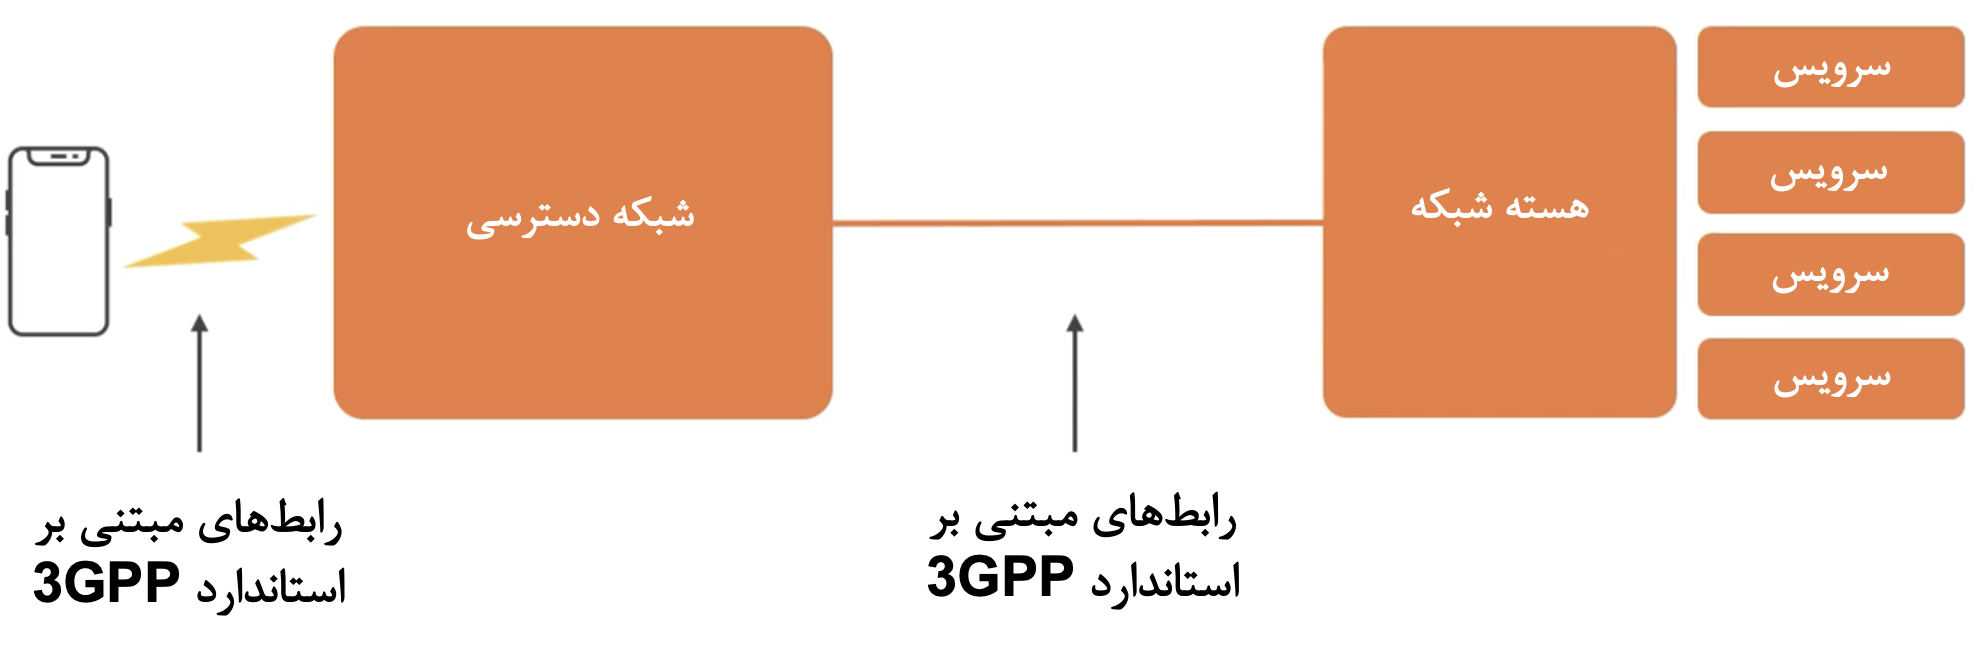
\includegraphics[width=\columnwidth]{Images/ran.png}
	\centering
	\caption{معماری کلی شبکه‌های تلفن همراه}
	\label{fig:ran}
\end{figure}

ناحیه دسترسی رادیویی مدت‌ها به صورت یک قسمت یک‌پارچه بوده و اطلاعاتی از کارهایی که درون آن انجام می‌شده به قسمت‌های دیگر برای بهینه‌سازی آن داده نمی‌شده و به طور کامل به تامین‌کنندگان وابسته بوده به طوری که برای داشتن یک ناحیه‌ی دسترسی رادیویی باید تمام تجهیزات آن را از یک تامین‌کننده تهیه می‌شده. 
\lr{3GPP}
به عنوان نهاد استاندارسازی شبکه‌های تلفن همراه در نسخه‌های جدیدی که از نسل پنجم شبکه‌های تلفن همراه 
(\lr{5G})
منتشر کرده‌است، ناحیه دسترسی رادیویی را جداسازی 
\LTRfootnote{Disaggregate}
کرده و آن را به ۳ قسمت تفکیک کرده‌است. در 
\ref{fig:3gpp-ran}
این ۳ قسمت قابل مشاهده‌ هستند. با این تفکیک و ایجاد قسمت‌های 
\lr{RU}
\lr{DU}،
و 
\lr{CU}
باید واسط‌های ارتباطی جدیدی برای ارتباط این قسمت‌ها تعریف می‌شد که این موارد نیز در این شکل مشاهده می‌شوند.
\begin{figure}
	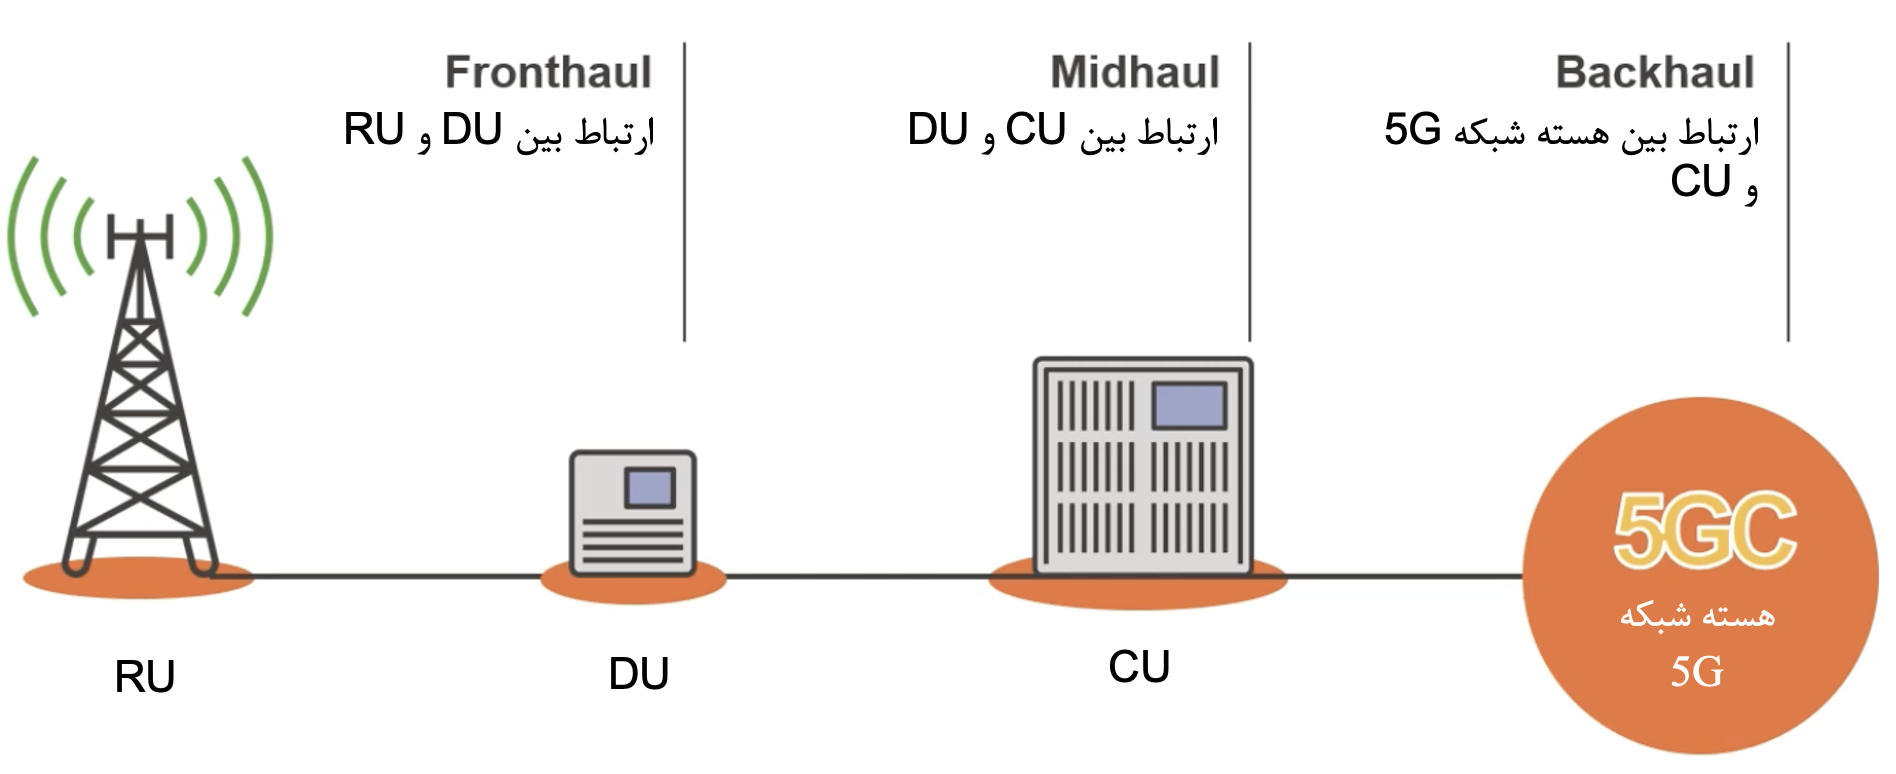
\includegraphics[width=\columnwidth]{Images/3gpp-ran.png}
	\centering
	\caption{تفکیک ناحیه‌ی رادیویی نسل ۵ توسط
		\lr{3GPP}}
	\label{fig:3gpp-ran}
\end{figure}

اگر عملکرد این قسمت‌های جدید را در پشته‌ی پروتکلی 
\LTRfootnote{Protocol Stack}
شبکه‌های تلفن همراه هم بررسی کنیم، می‌توانیم وظایف موجود در هر کدام از لایه‌های مختلف را به یکی از این قسمت‌های جدید در ناحیه دسترسی رادیویی واگذار کنیم.

در ادامه‌ی این راه و برای توسعه‌ی بیش‌تر این رویکرد جدید در ناحیه‌ی دسترسی رادیویی، سازمانی تحت عنوان
\lr{O-RAN Alliance} 
تشکیل شد که هدف آن تمرکز بر همین ایده و پیش‌برد ناحیه‌ی دسترسی رادیویی‌ای آزادتر و هوشمندتر بود.

\begin{figure}[H]
	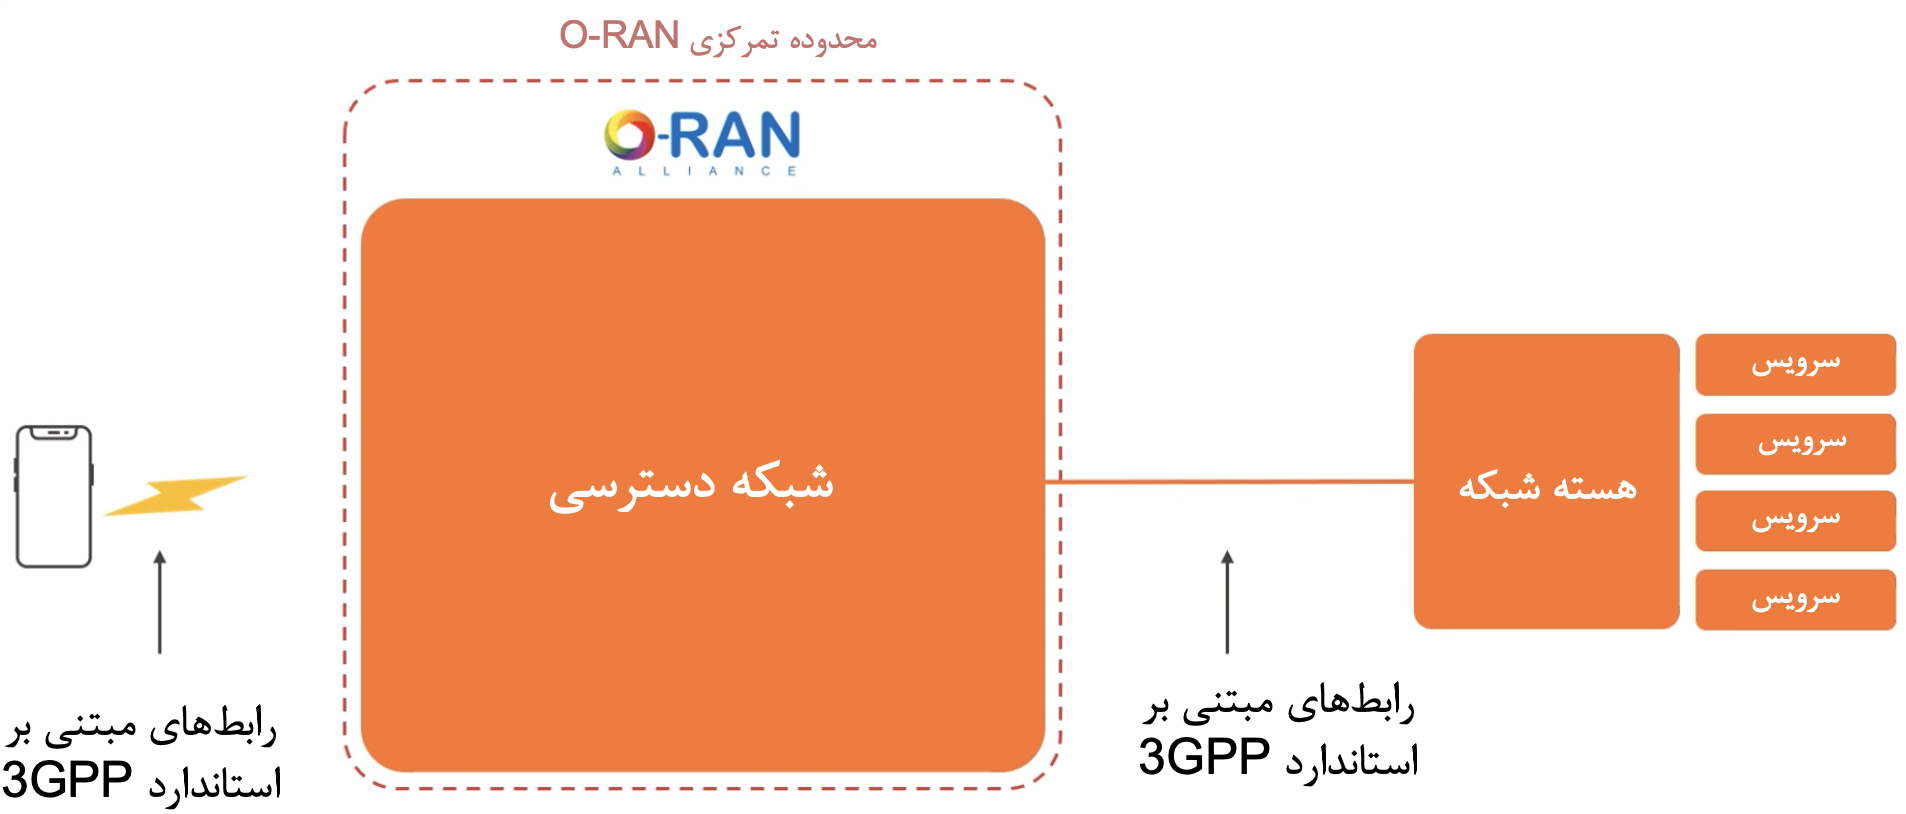
\includegraphics[width=\columnwidth]{Images/alliance.png}
	\centering
	\caption{تمرکز کاری
		\lr{O-RAN Alliance}}
	\label{fig:alliance}
\end{figure}

در بخش‌های بعدی، معماری 
\lr{O-RAN} 
بررسی شده. 
\section{مروری بر کارهای پیشین}
برای تهیه‌ی این گزارش از چندین مقاله استفاده شده است.
\cite{polese2023understanding}
که یک مقاله‌ی مروری و آموزشی است و تقریبا اکثر مفاهیم موجود در مورد معماری 
\lr{O-RAN}
و بخش‌های مختلف 
\lr{RIC}
در آن توضیح داده شده‌است که مفاهیم آن در بخش‌های بعدی این گزارش بیان شده‌اند. در
\cite{upadhyaya2022prototyping}
به این مسئله پرداخته شده که شبکه‌های تلفن همراه سال‌ها در تسخیر تامین‌کنندگان بوده‌ و راهکار مناسبی برای انجام پژوهش و آزمایش‌های متنوع بر روی این شبکه‌ها میسر نبوده اما با معرفی معماری
\lr{O-RAN}،
این انحصار از بین رفته و در این مقاله هم تلاش شده علاوه بر توضیح این معماری، بستری به عنوان محیط تستی برای انجام آزمایش‌ها و بهینه‌سازی‌های مختلف آماده شود که در آن به کمک این معماری و هم‌چنین استفاده از اجزای نرم‌افزاری-رادیویی
\LTRfootnote{Software-defined radio (SDR)}
، بتوان به بهبود نسل پنجم شبکه‌های تلفن همراه پرداخت. در حقیقت یک شبکه‌ی نسل پنجم کامل و بدون وابستگی به تامین‌کننده‌ی خاصی در این مقاله پیاده‌سازی شده و به مفاهیم به صورت کاربردی‌تر پرداخته شده. در این مقاله بیان شده که کاربرد 
\lr{xApp}هایی
که در بخش
\lr{RIC}
معماری 
\lr{O-RAN}
قرار می‌گیرند می‌تواند به صورت کنترلی یا نظارتی باشد. در نهایت هم یک
\lr{xApp}
برای تقسیم‌بندی پهنای باند سلولی یعنی با اهداف کنترلی و هم‌چنین یک 
\lr{xApp}
دیگر برای پایش وضعیت شبکه یعنی با اهداف نظارتی پیاده‌سا‌زی شده. جریان کاری یکی از این 
\lr{xApp}ها
که وظیفه‌اش پایش وضعیت شبکه است را در 
\begin{figure*}
	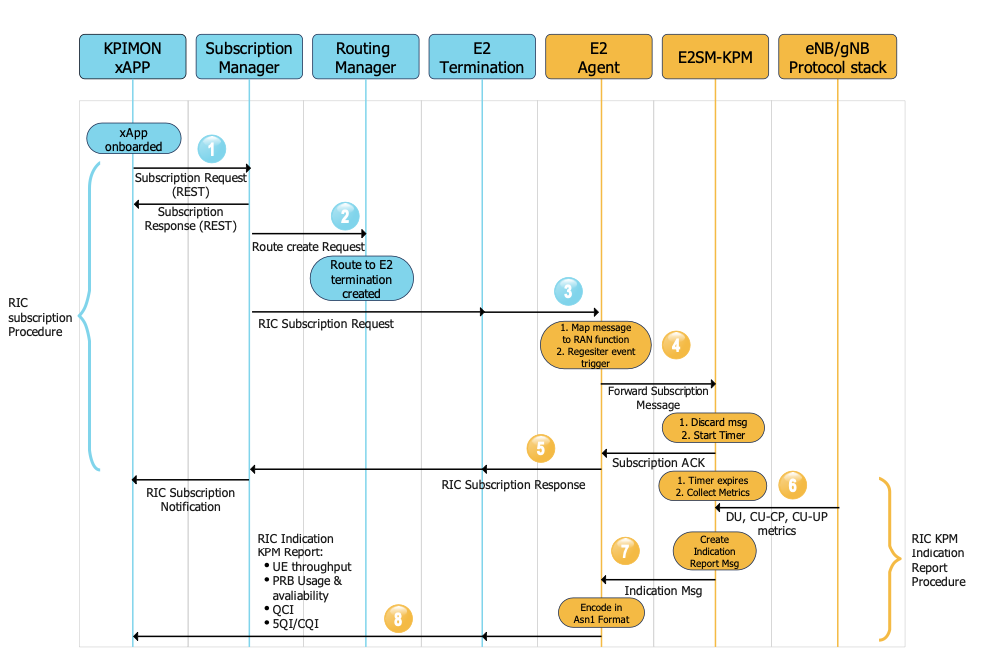
\includegraphics[width=\linewidth]{Images/kpimon.png}
	\centering
	\caption{جریان انتها به انتهای عملکردی یک
	\lr{xApp}
	برای پایش وضعیت شبکه
\cite{upadhyaya2022prototyping}
}
	\label{fig:kpimon}
\end{figure*}
می‌توان دید که توضیحات قسمت‌های مختلف آن در بخش مفاهیم به طور کامل بیان شده است.
در
\cite{orhan2021connection}
به صورت دقیق‌تر به سراغ اهداف بهینه‌سازی رفته‌اند و تلاش شده با استفاده از الگوریتم‌های هوش مصنوعی به بهبود وضعیت شبکه بپردازند. در این تحقیق به کمک شبکه‌های عصبی عمیق گرافی 
\LTRfootnote{Deep Graph Neural Networks}
و هم‌چنین یادگیری تقویتی
\LTRfootnote{Reinforcement Learning}
به مدیریت اتصال‌های شبکه پرداخته شده و تلاش شده تا با کمک این روش‌ها، علاوه بر تجربه‌ی کیفیت مناسب در اتصال دستگاه‌ها به آنتن، اتصال‌ها نیز به صورت همگن‌تری بین گره‌های مختلف شبکه پخش شود. 

\section{بیان مفاهیم}

\subsection{معماری
\lr{O-RAN}
}

ساختاری که در 
\lr{O-RAN}
معرفی شده در 
\ref{fig:oran}
قابل مشاهده است. همان‌طور که می‌بینیم علاوه بر قسمت‌هایی که 
\lr{3GPP}
در ناحیه‌ی دسترسی رادیویی تعبیه کرده بود، قسمت‌های جدیدی هم به آن اضافه شده‌اند 

\begin{figure*}
	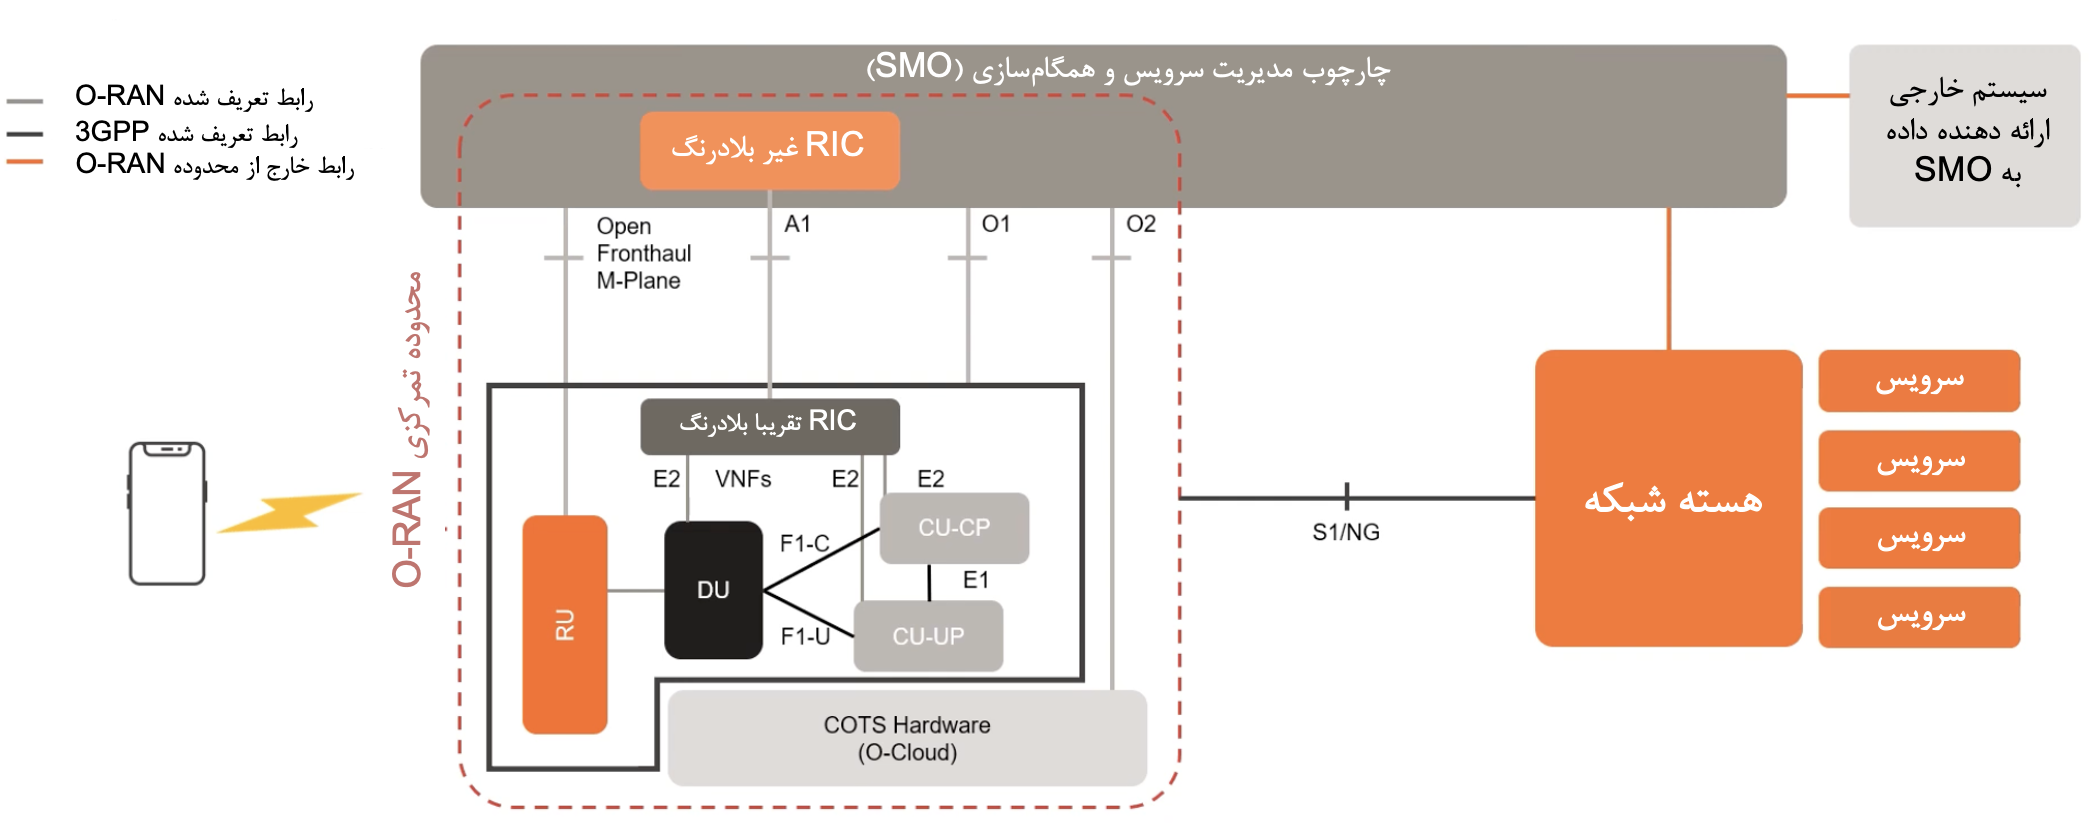
\includegraphics[width=\linewidth]{Images/oran.png}
	\centering
	\caption{ساختار کلی شبکه‌های تلفن همراه با
		\lr{O-RAN}}
	\label{fig:oran}
\end{figure*}

می‌بینیم که علاوه بر 
\lr{RU}
\lr{DU}،
و 
\lr{CU}،
قسمت‌های جدیدی مانند 
\lr{Near Real-Time (RT) RIC}
و 
\lr{None Real-Time (RT) RIC}
اضافه شده که این قسمت‌های جدید برای کنترل ناحیه‌ی دسترسی رادیویی به صورت هوشمندانه هستند که در فصل‌های بعدی بررسی شده اند.

در 
\lr{Near-RT RIC}
تمرکز بر کنترل به صورت نزدیک به بلادرنگ است و در 
\lr{None-RT RIC}
کنترل‌های با تاخیر بالاتر از یک ثانیه انجام می‌گیرد. 

\subsection{\lr{Near-RT RIC}}

یکی از اجزای اصلی
\lr{O-RAN}،
\lr{Near-RT RIC} 
است که وظیفه‌ی کنترل هوشمندانه‌ی ناحیه دسترسی رادیویی با تاخیر نسبتا کم و به صورت نزدیک به بلادرنگ (بین ۱۰ میلی‌ثانیه تا ۱ ثانیه) را برعهده دارد.

این قسمت همان‌طور که در 
\ref{fig:nrt-ric0}
هم مشاهده می‌شود، خود از قسمت‌های زیادی تشکیل شده که در ادامه هر کدام از آن‌ها معرفی خواهند شد.

\begin{figure}[H]
	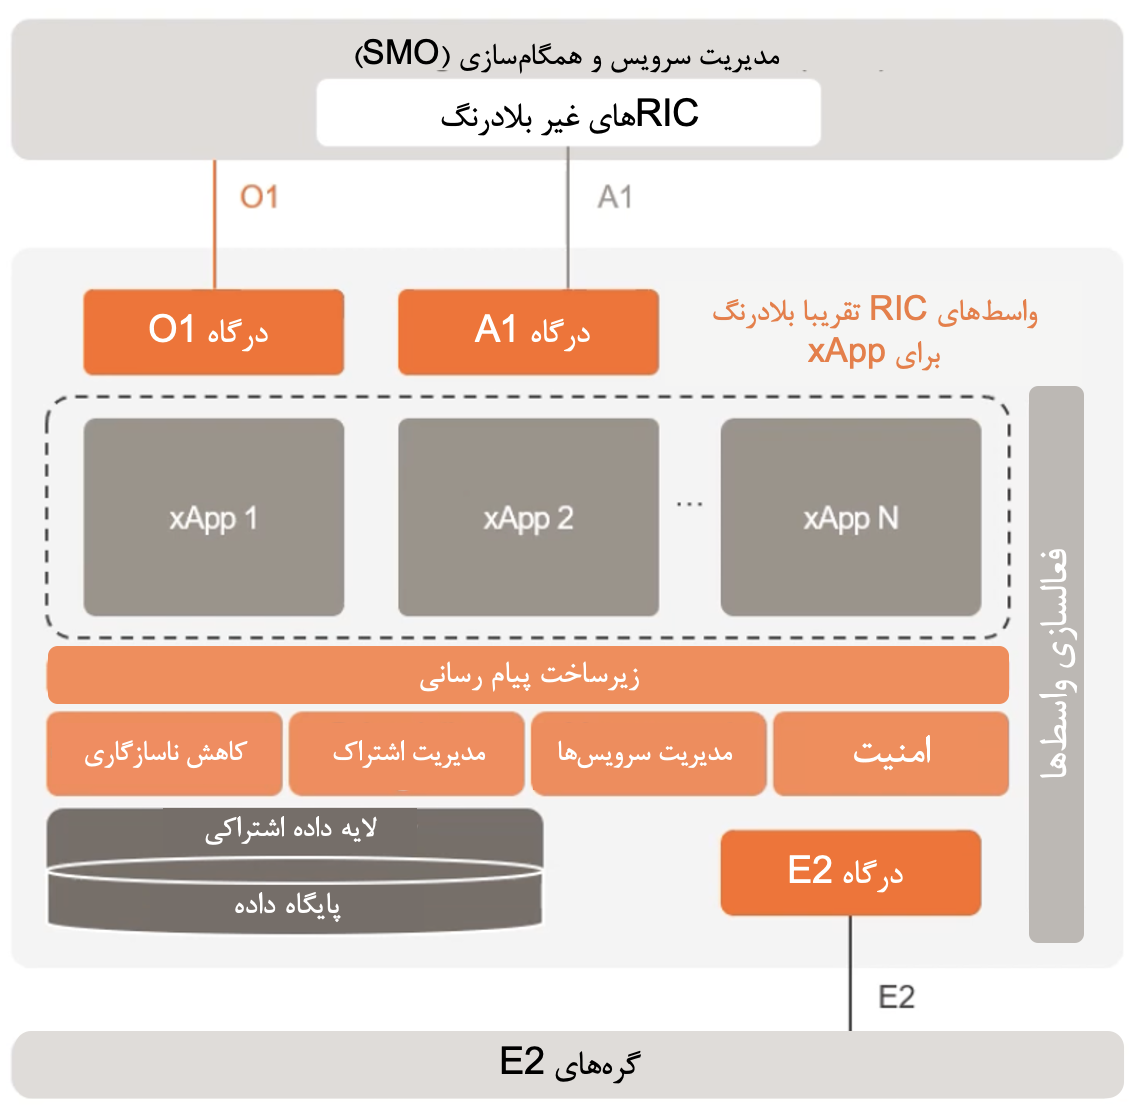
\includegraphics[width=\columnwidth]{Images/nrt-ric0.png}
	\centering
	\caption{اجزای مختلف موجود در
		\lr{Near-RT RIC}}
	\label{fig:nrt-ric0}
\end{figure}

\subsubsection{\lr{xApp}}
اصلی‌ترین مفهوم در 
\lr{Near-RT RIC}، 
\lr{xApp} 
است. 
\lr{xApp}ها
یک سری برنامه‌ی کوچک اند که یکی از اصلی‌ترین کاربردهای آن‌ها به این صورت است که از طریق آن‌ها تصمیم‌های کنترلی به کمک داده‌هایی که به عنوان ورودی به آن‌ها داده می‌شود، گرفته می‌شود. این تصمیم‌ها از طریق واسط
\lr{E2}
که در بخش‌‌های بعدی معرفی می‌شود، به دست گره‌های 
\lr{E2}
که همان
\lr{DU} یا
\lr{CU}
هستند، می‌رسد تا اجرایی شوند.


\subsubsection{زیرساخت پیام‌رسانی}
این بخش یک زیرساخت پیام‌رسانی است که پیغام‌های مختلف بین اجزای مختلف موجود در
\lr{Near-RT RIC} 
از طریق آن رد و بدل می‌شود. 

\subsubsection{کاهش تعارض‌ها}
این بخش وظیفه دارد تا از بروز اشکالاتی که به خاطر تداخل پیکره‌بندی‌های مختلفی که 
\lr{xApp}ها
به وجود می‌آورند جلوگیری کند یا اینکه با مکانیزم‌های خود، آن‌ها را تشخیص دهد و سپس آن‌ها را اصلاح کند. به صورت ساده‌تر این قسمت از دست‌کاری موارد یکسان توسط برنامه‌های مختلف که ممکن است باعث خرابی عملکردی شود، جلوگیری می‌کند.

\subsubsection{مدیریت اشتراک‌ها}
این بخش بررسی و مدیریت اینکه
\lr{xApp}های
مختلف به گره‌های
\lr{E2}ی
که می‌خواهند اطلاعات از آن‌ها دریافت کند، درخواستشان را ارسال کنند را برعهده دارد. به عنوان مثال اگر چندین برنامه نیازمند به یک مرجع داده‌ی یکسان داشته باشند، این بخش این درخواست‌ها را تجمیع می‌کند تا مدیریت و کنترل‌ آن‌ها ساده‌تر باشد.

\subsubsection{مدیریت سرویس‌ها}
این بخش وظیفه‌ی مدیریت خود
\lr{xApp}ها،
ساختار عیب‌یابی و عملیاتی کردن آن‌ها و به صورت کلی موارد مرتبط با خود 
\lr{xApp}ها
را بر عهده دارد.

\subsubsection{امنیت}
با توجه به اینکه اطلاعات موجود در ناحیه‌ی دسترسی رادیویی، اطلاعات محرمانه‌ای در مورد کاربران را شامل می‌شود، این قسمت وظیفه‌اش حفظ امنیت این داده‌ها است. البته هنوز در پیاده‌سازی‌هایی که انجام شده به سراغ این موضوع به صورت جدی نرفته‌اند و در دست پیشرفت است.

\subsubsection{پایگاه داده}
این قسمت هم، همان‌طور که نامش پیداست،‌ پایگاه داده‌ای است که اطلاعات مختلف کاربران را نگه‌داری می‌کند تا 
\lr{xApp}های
مختلف در صورت نیاز بتوانند از آن‌ها استفاده کنند و دستورات کنترلی لازم را صادر کنند.


\subsubsection{درگاه‌ها}
در شکل چندین درگاه مختلف آورده شده که از طریق آن‌ها،
\lr{Near-RT RIC} 
به بخش‌های دیگر موجود در 
\lr{O-RAN}
پیغام رد و بدل می‌کند. در بخش‌های بعدی با جزئیات بیش‌تری در مورد هر کدام از آن‌ها صحبت به میان آورده شده‌است.

\subsection{\lr{None-RT RIC}}

بخش بعدی‌ای که در 
\lr{O-RAN}
به ناحیه‌ی رادیویی اضافه شده‌است را با این توضیح آغاز می‌کنیم که طبق 
\ref{fig:nonert-ric1}،
قسمت مهم 
\lr{None-RT RIC}
که وظیفه‌ی دادن فرمان‌های کنترلی با تاخیرهای بیش‌تر از یک ثانیه است، داخل بخش دیگری به نام
\lr{SMO}
قرار می‌گیرد که خود از قسمت‌های مختلفی تشکیل شده‌است و وظایف گوناگونی را بر عهده دارد. کارهایی که در این بخش صورت می‌گیرد، وظایف سطح بالاتری نسبت به وظایف موجود در 
\lr{Near-RT RIC}
است.

\begin{figure}
	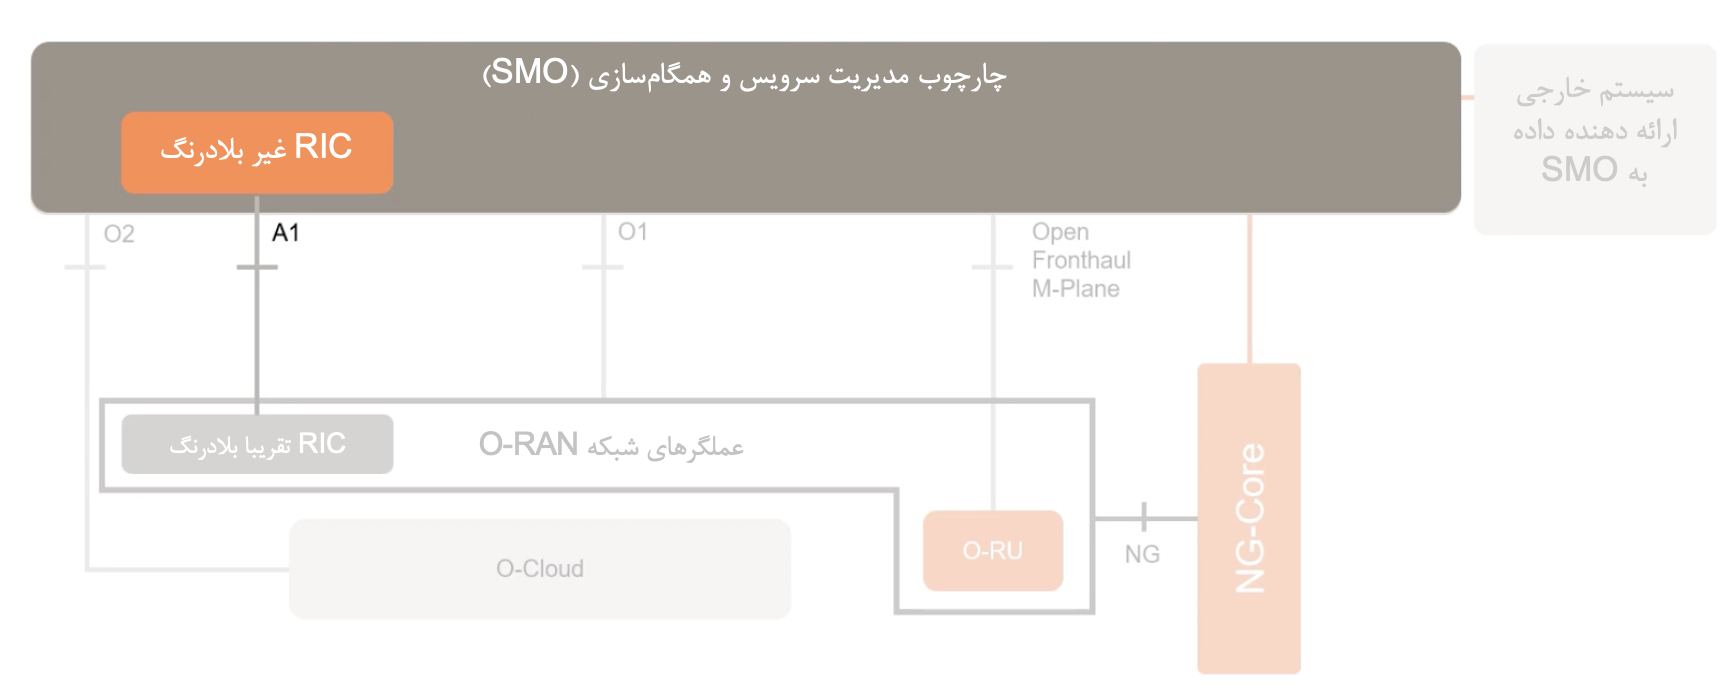
\includegraphics[width=\columnwidth]{Images/nonert-ric1.png}
	\centering
	\caption{اجزای مختلف موجود در
		\lr{Near-RT RIC}}
	\label{fig:nonert-ric1}
\end{figure}

در 
\ref{fig:nonert-ric2}
جزئی‌تر به
\lr{SMO}
پرداخته شده و بخش‌های مختلف آن به نمایش کشیده شده‌است.

به صورت کلی
\lr{SMO}
به سه بخش تقسیم می‌شود.

بخش اول همان قسمتی است که با عنوان 
\lr{None-RT RIC}
شناخته می‌شود که خود آن از تعدادی
\lr{rApp}
تشکیل شده‌است. این
\lr{rApp}ها
برنامه‌هایی شبیه به 
\lr{xApp}ها 
هستند با این تفاوت که در بخش 
\lr{None-RT RIC}
حضور دارند.

بخش دوم هم قسمتی است که خارج از
\lr{None-RT RIC}
قرار می‌گیرد و کارهای مدیریتی درون 
\lr{SMO}
و موارد مرتبط با خودکارسازی و پیکره‌بندی را برعهده دارد.

\begin{figure}
	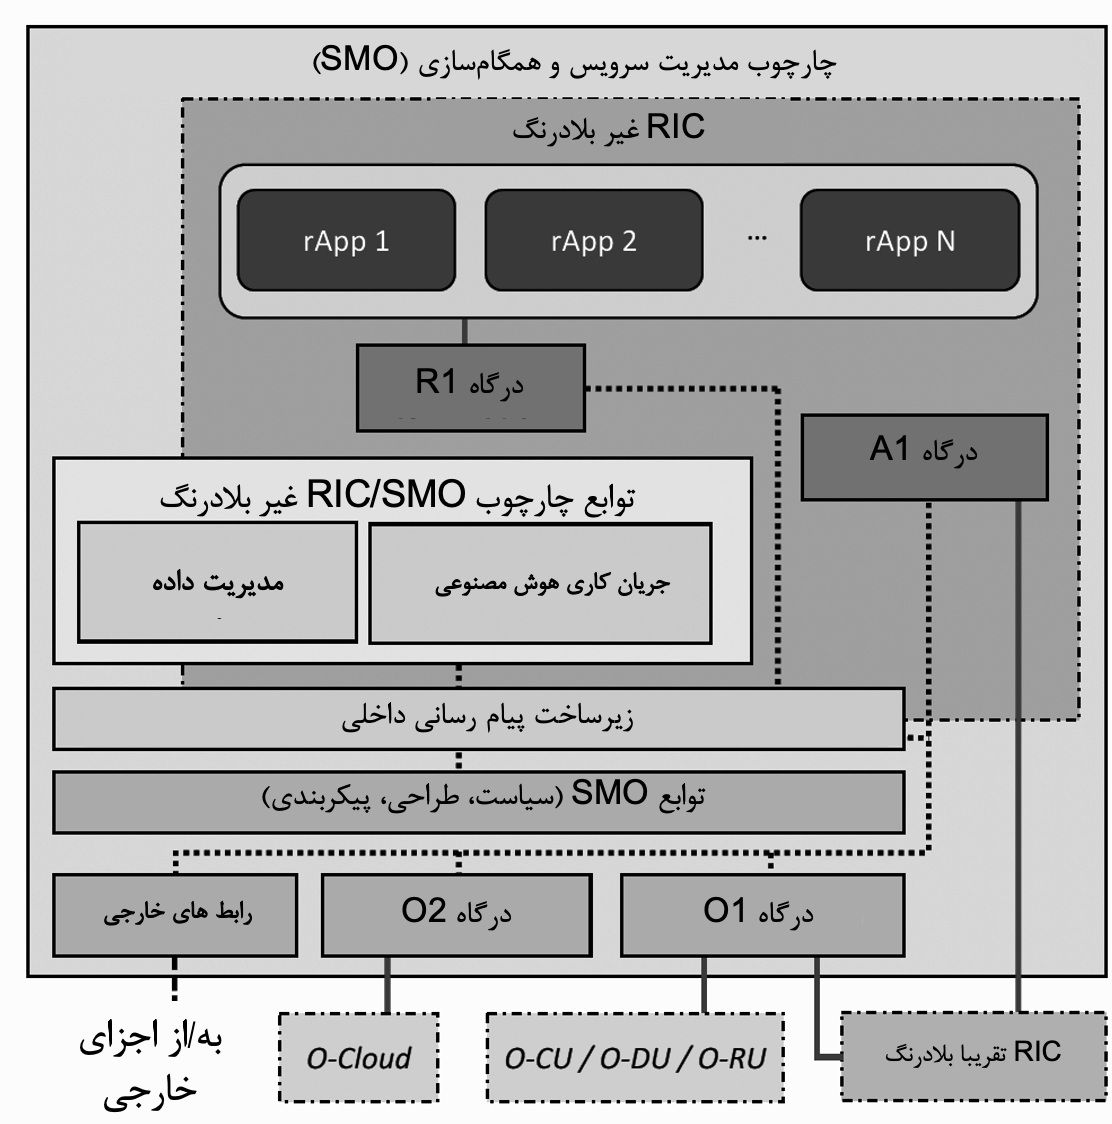
\includegraphics[width=\columnwidth]{Images/nonert-ric2.png}
	\centering
	\caption{اجزای مختلف موجود در
		\lr{Near-RT RIC}}
	\label{fig:nonert-ric2}
\end{figure}

بخش سوم نیز قسمت میانی‌ای است که بین
\lr{SMO}
و
\lr{None-RT RIC}
قرار دارد و قسمتی از آن به ساختار دادن به دادگان و جمع‌آوری آن‌ها اختصاص دارد تا بتوان در قسمت‌های داده‌محور از آن‌ها استفاده کرد و بخش دیگر جریان یادگیری ماشین را در خود جای داده‌است.

جریان کاری یادگیری ماشین از قسمت‌های مختلفی مانند جمع‌آوری و آماده‌سازی دادگان، آموزش مدل یادگیری ماشین، اعتبار سنجی آن و بالا آوردن آن در محیط عملیاتی و هم‌چنین بهبود پیوسته‌ی آن تشکیل شده است. البته همه‌ی این موارد به طور کامل می‌تواند در این قسمت از 
\lr{SMO}
جایگذاری نشود و با توجه به سناریوهای مختلف، هر کدام از این مراحل در بخش‌های مختلف 
\lr{O-RAN}
مانند 
\lr{xApp}ها
قرار گیرد.

\subsection{واسط‌ها}

\begin{figure*}
	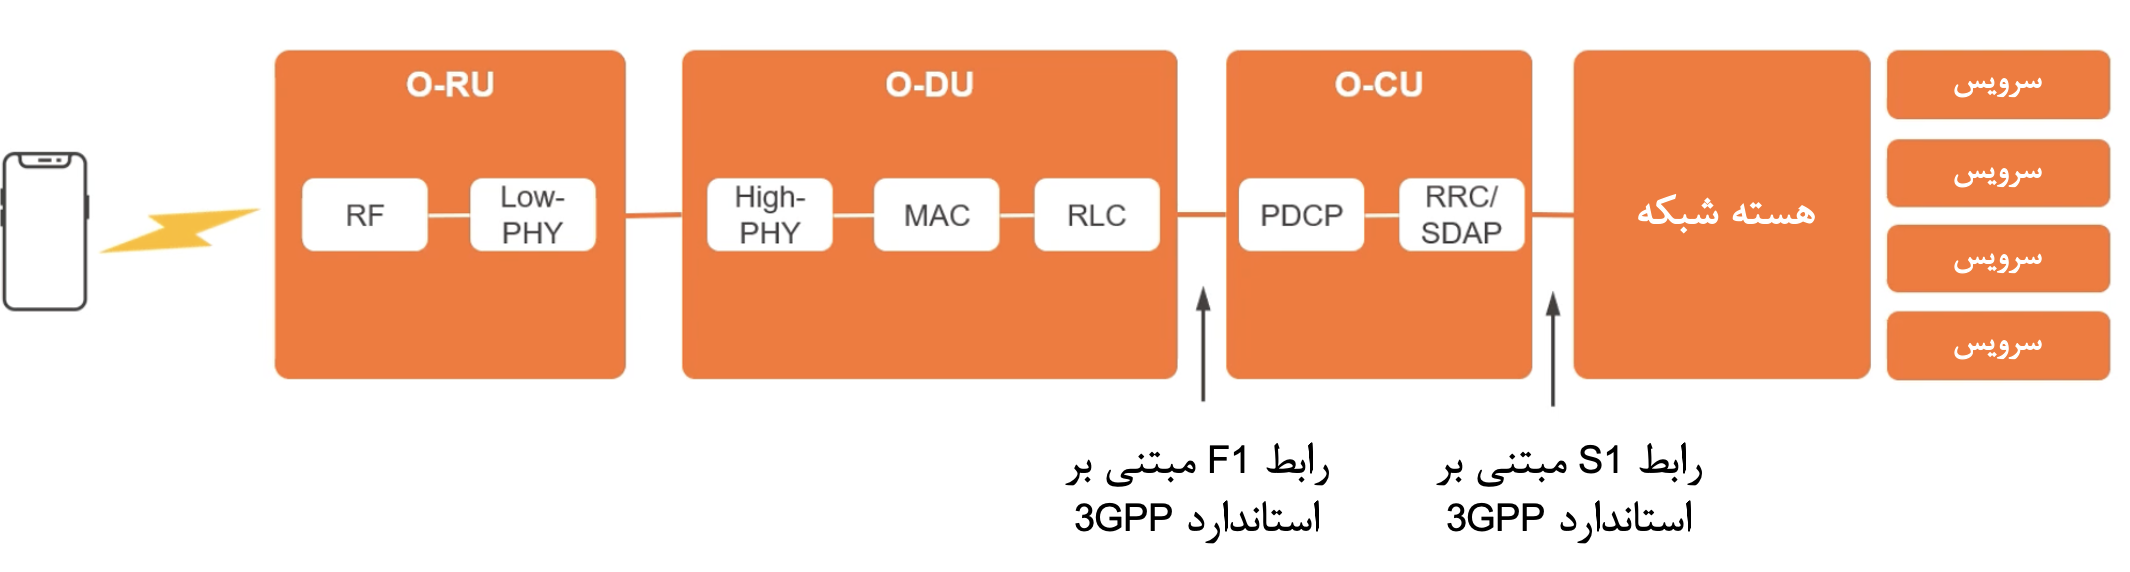
\includegraphics[width=\linewidth]{Images/int1.png}
	\centering
	\caption{واسط‌های معرفی شده توسط
		\lr{3GPP}}
	\label{fig:int1}
\end{figure*}
با توجه به معرفی اجزای جدید در معماری 
\lr{O-RAN}
این نیاز وجود دارد که برای ارتباط بین قسمت‌های مختلف، واسط‌های به صورت استاندارد تعریف شود تا بتوان برنامه‌های مختلفی توسعه داد و اجزای مختلف هم بتوانند به درستی با کمک این واسط‌های استاندارد شده با یک‌دیگر ارتباط برقرار کنند و دیگر همه چیز در اختیار تامین‌کنندگان قطعات نباشد.

در ادامه واسط‌های مختلفی که در 
\ref{fig:nrt-ric0}
 دیدیم بررسی شده‌اند.

بعضی از این واسط‌ها توسط 
\lr{3GPP}
استاندارد شده‌اند که در 
\ref{fig:int1}
هم آورده شده‌اند. 

واسط
\lr{F1}
برای ارتباط بین
\lr{DU}
و
\lr{CU}
آماده شده است.

واسط
\lr{S1}
برای ارتباط بین
\lr{CU}
و هسته‌ی شبکه معرفی شده است. 

در ادامه به بررسی واسط‌های اختصاصی
\lr{O-RAN} 
پرداخته شده. واسط
\lr{E2}
برای ارتباط بین
\lr{Near-RT RIC}ها
با 
\lr{CU}
و
\lr{DU}
در نظر گرفته شده است. واسط
\lr{A1}
برای ارتباط بین
\lr{Near-RT RIC}
و 
\lr{None-RT RIC}
معرفی شده است. واسط
\lr{O1}
برای ارتباط بین
\lr{SMO}
‌و اجزای مختلف اختصاصی 
\lr{O-RAN}
در نظر گرفته شده است.

در آخر هم در 
\ref{fig:sample}
می‌توانیم نمونه‌ای از ارتباط بین یک گره‌
\lr{E2}
و
\lr{Near-RT RIC}
را از طریق واسط
\lr{E2}
ببینیم به این صورت که ابتدا از طریق بخش مدیریت اشتراک که در مفاهیم توضیح داده شد، درخواست دریافت داده‌ی خاصی از سمت 
\lr{Near-RT RIC}
به گره
\lr{E2}
می‌شود. ممکن است این اشتراک برای یک مورد پایشی باشد و به صورت دوره‌ای ارسال شود یا اینکه ممکن است این داده بر اثر وقوع رخدادها ارسال شود و این اشتراک برای دادن دستورهای کنترلی بوده باشد که در این حالت این گره اطلاعات مورد نظر را برای 
\lr{Near-RT RIC}
ارسال می‌کند. اگر این داده نیازمند دریافت تصمیمی از سوی 
\lr{RIC}
باشد، گره
\lr{E2}
مدت زمان مشخصی را برای این تصمیم صبر می‌کند و اگر دستوری دریافت کند، آن را اجرا می‌کند و در صورت عدم دریافت پاسخ، خودش بدون کمک 
\lr{RIC}
تصمیم‌گیری می‌کند. به عنوان مثال این تصمیم می‌تواند تصمیم‌گیری برای تحویل‌دادن یک کاربر به یک سلول دیگر
(\lr{Handover})
باشد.

\begin{figure*}
	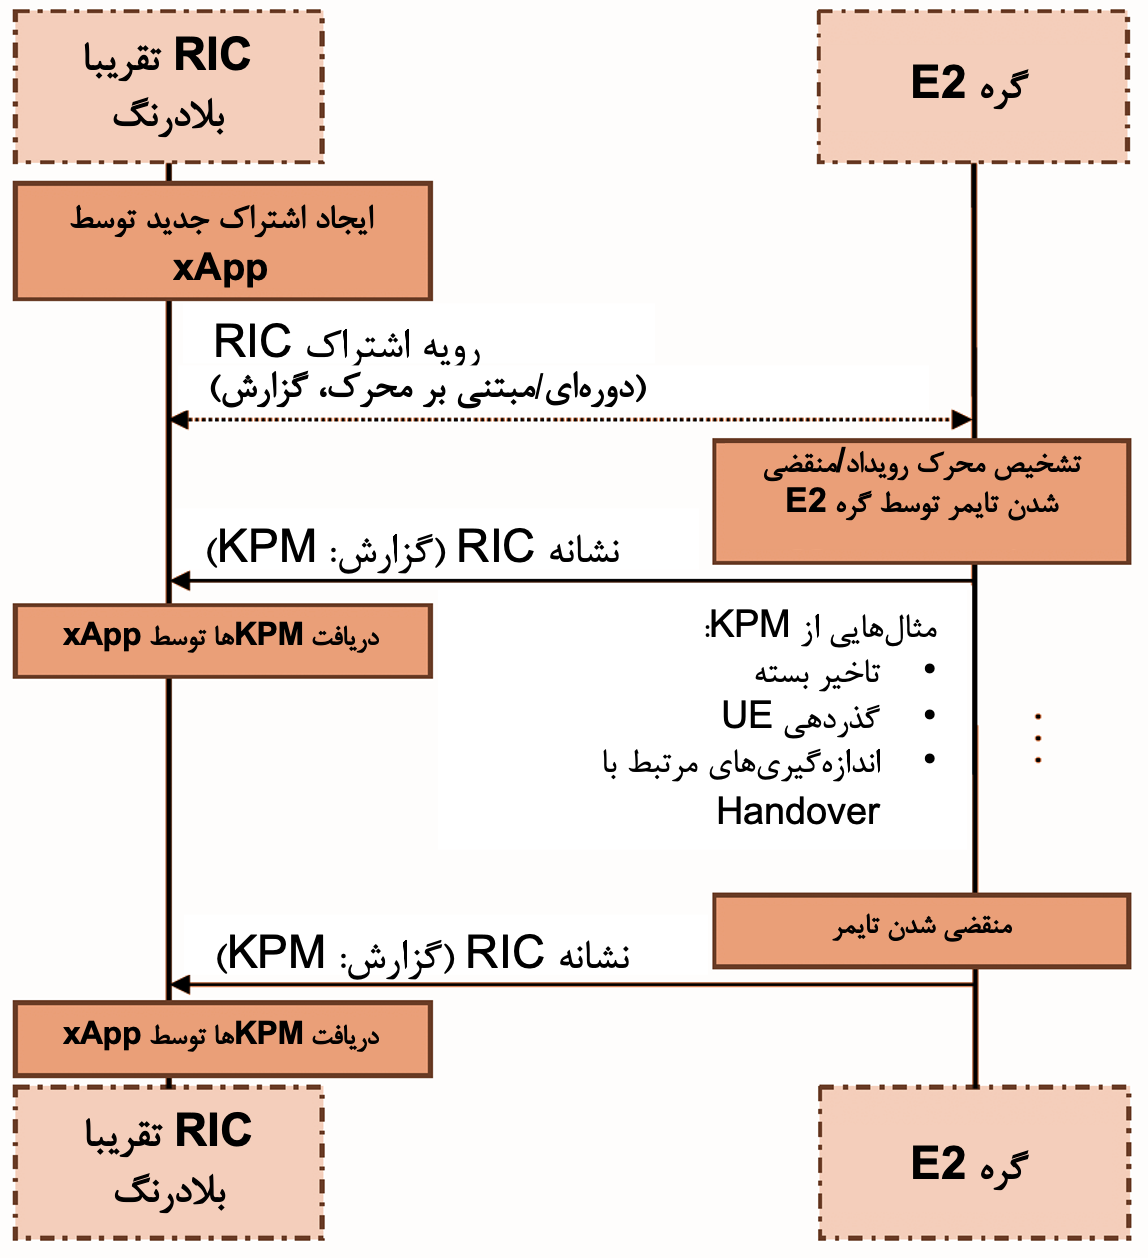
\includegraphics[width=0.6\linewidth]{Images/sample.png}
	\centering
	\caption{نمونه‌ای از ارتباط بین گره
\lr{E2}
و
\lr{Near-RT RIC}	
}
	\label{fig:sample}
\end{figure*}


\section{نتیجه گیری}

در این گزارش هدف نهایی این بود که با کاربرد 
\lr{RIC}
در کنترل و بهینه‌سازی شبکه‌های نسل پنجم تلفن همراه آشنا شویم و دیدیم که 
\lr{RIC}
قسمتی از معماری جدیدی در شبکه‌های تلفن همراه به نام
\lr{O-RAN}
است که با هدف از بین بردن انحصار ناحیه‌ی رادیویی شبکه‌های تلفن همراه از دست تامین‌کنندگان و هم‌چنین هوشمند‌تر کردن این ناحیه معرفی شده و هم‌چنین بسیاری از بخش‌های آن با کمک روش‌های نرم‌افزاری و مجازی‌سازی، قابلیت مقیاس‌پذیری به آن داده است. همان‌طور که بیان شد، ناحیه‌ی 
\lr{RAN} 
به کمک رابط‌ جدیدی به نام
\lr{E2}
که در این معماری معرفی شده، با 
\lr{xApp}های 
پیاده‌سازی شده در 
\lr{Near-RT RIC}
که می‌توانند از روش‌های داده‌محور استفاده کنند، ارتباط برقرار می‌کند و می‌‌تواند از تصمیمات این بخش برای بهبود وضعیت شبکه استفاده کند. 

\bibliography{lib}

\theendnotes
\end{document}


